\documentclass[11pt,a4paper]{report}
\usepackage[textwidth=37em,vmargin=30mm]{geometry}
\usepackage{calc,xunicode,amsmath,amssymb,paralist,enumitem,tabu,booktabs,datetime2,xeCJK,xeCJKfntef,listings}
\usepackage{tocloft,fancyhdr,tcolorbox,xcolor,graphicx,eso-pic,xltxtra,xelatexemoji}

\newcommand{\envyear}[0]{2025}
\newcommand{\envdatestr}[0]{2025-08-20}
\newcommand{\envfinaldir}[0]{webdb/2025/20250820/final}

\usepackage[hidelinks]{hyperref}
\hypersetup{
    colorlinks=false,
    pdfpagemode=FullScreen,
    pdftitle={Web Digest - \envdatestr}
}

\setlength{\cftbeforechapskip}{10pt}
\renewcommand{\cftchapfont}{\rmfamily\bfseries\large\raggedright}
\setlength{\cftbeforesecskip}{2pt}
\renewcommand{\cftsecfont}{\sffamily\small\raggedright}

\setdefaultleftmargin{2em}{2em}{1em}{1em}{1em}{1em}

\usepackage{xeCJK,xeCJKfntef}
\xeCJKsetup{PunctStyle=plain,RubberPunctSkip=false,CJKglue=\strut\hskip 0pt plus 0.1em minus 0.05em,CJKecglue=\strut\hskip 0.22em plus 0.2em}
\XeTeXlinebreaklocale "zh"
\XeTeXlinebreakskip = 0pt


\setmainfont{Brygada 1918}
\setromanfont{Brygada 1918}
\setsansfont{IBM Plex Sans}
\setmonofont{JetBrains Mono NL}
\setCJKmainfont{Noto Serif CJK SC}
\setCJKromanfont{Noto Serif CJK SC}
\setCJKsansfont{Noto Sans CJK SC}
\setCJKmonofont{Noto Sans CJK SC}

\setlength{\parindent}{0pt}
\setlength{\parskip}{8pt}
\linespread{1.15}

\lstset{
	basicstyle=\ttfamily\footnotesize,
	numbersep=5pt,
	backgroundcolor=\color{black!5},
	showspaces=false,
	showstringspaces=false,
	showtabs=false,
	tabsize=2,
	captionpos=b,
	breaklines=true,
	breakatwhitespace=true,
	breakautoindent=true,
	linewidth=\textwidth
}






\newcommand{\coverpic}[2]{
    % argv: itemurl, authorname
    Cover photo by #2~~(\href{#1}{#1})
}
\newcommand{\makeheader}[0]{
    \begin{titlepage}
        % \newgeometry{hmargin=15mm,tmargin=21mm,bmargin=12mm}
        \begin{center}
            
            \rmfamily\scshape
            \fontspec{BaskervilleF}
            \fontspec{Old Standard}
            \fontsize{59pt}{70pt}\selectfont
            WEB\hfill DIGEST
            
            \vfill
            % \vskip 30pt
            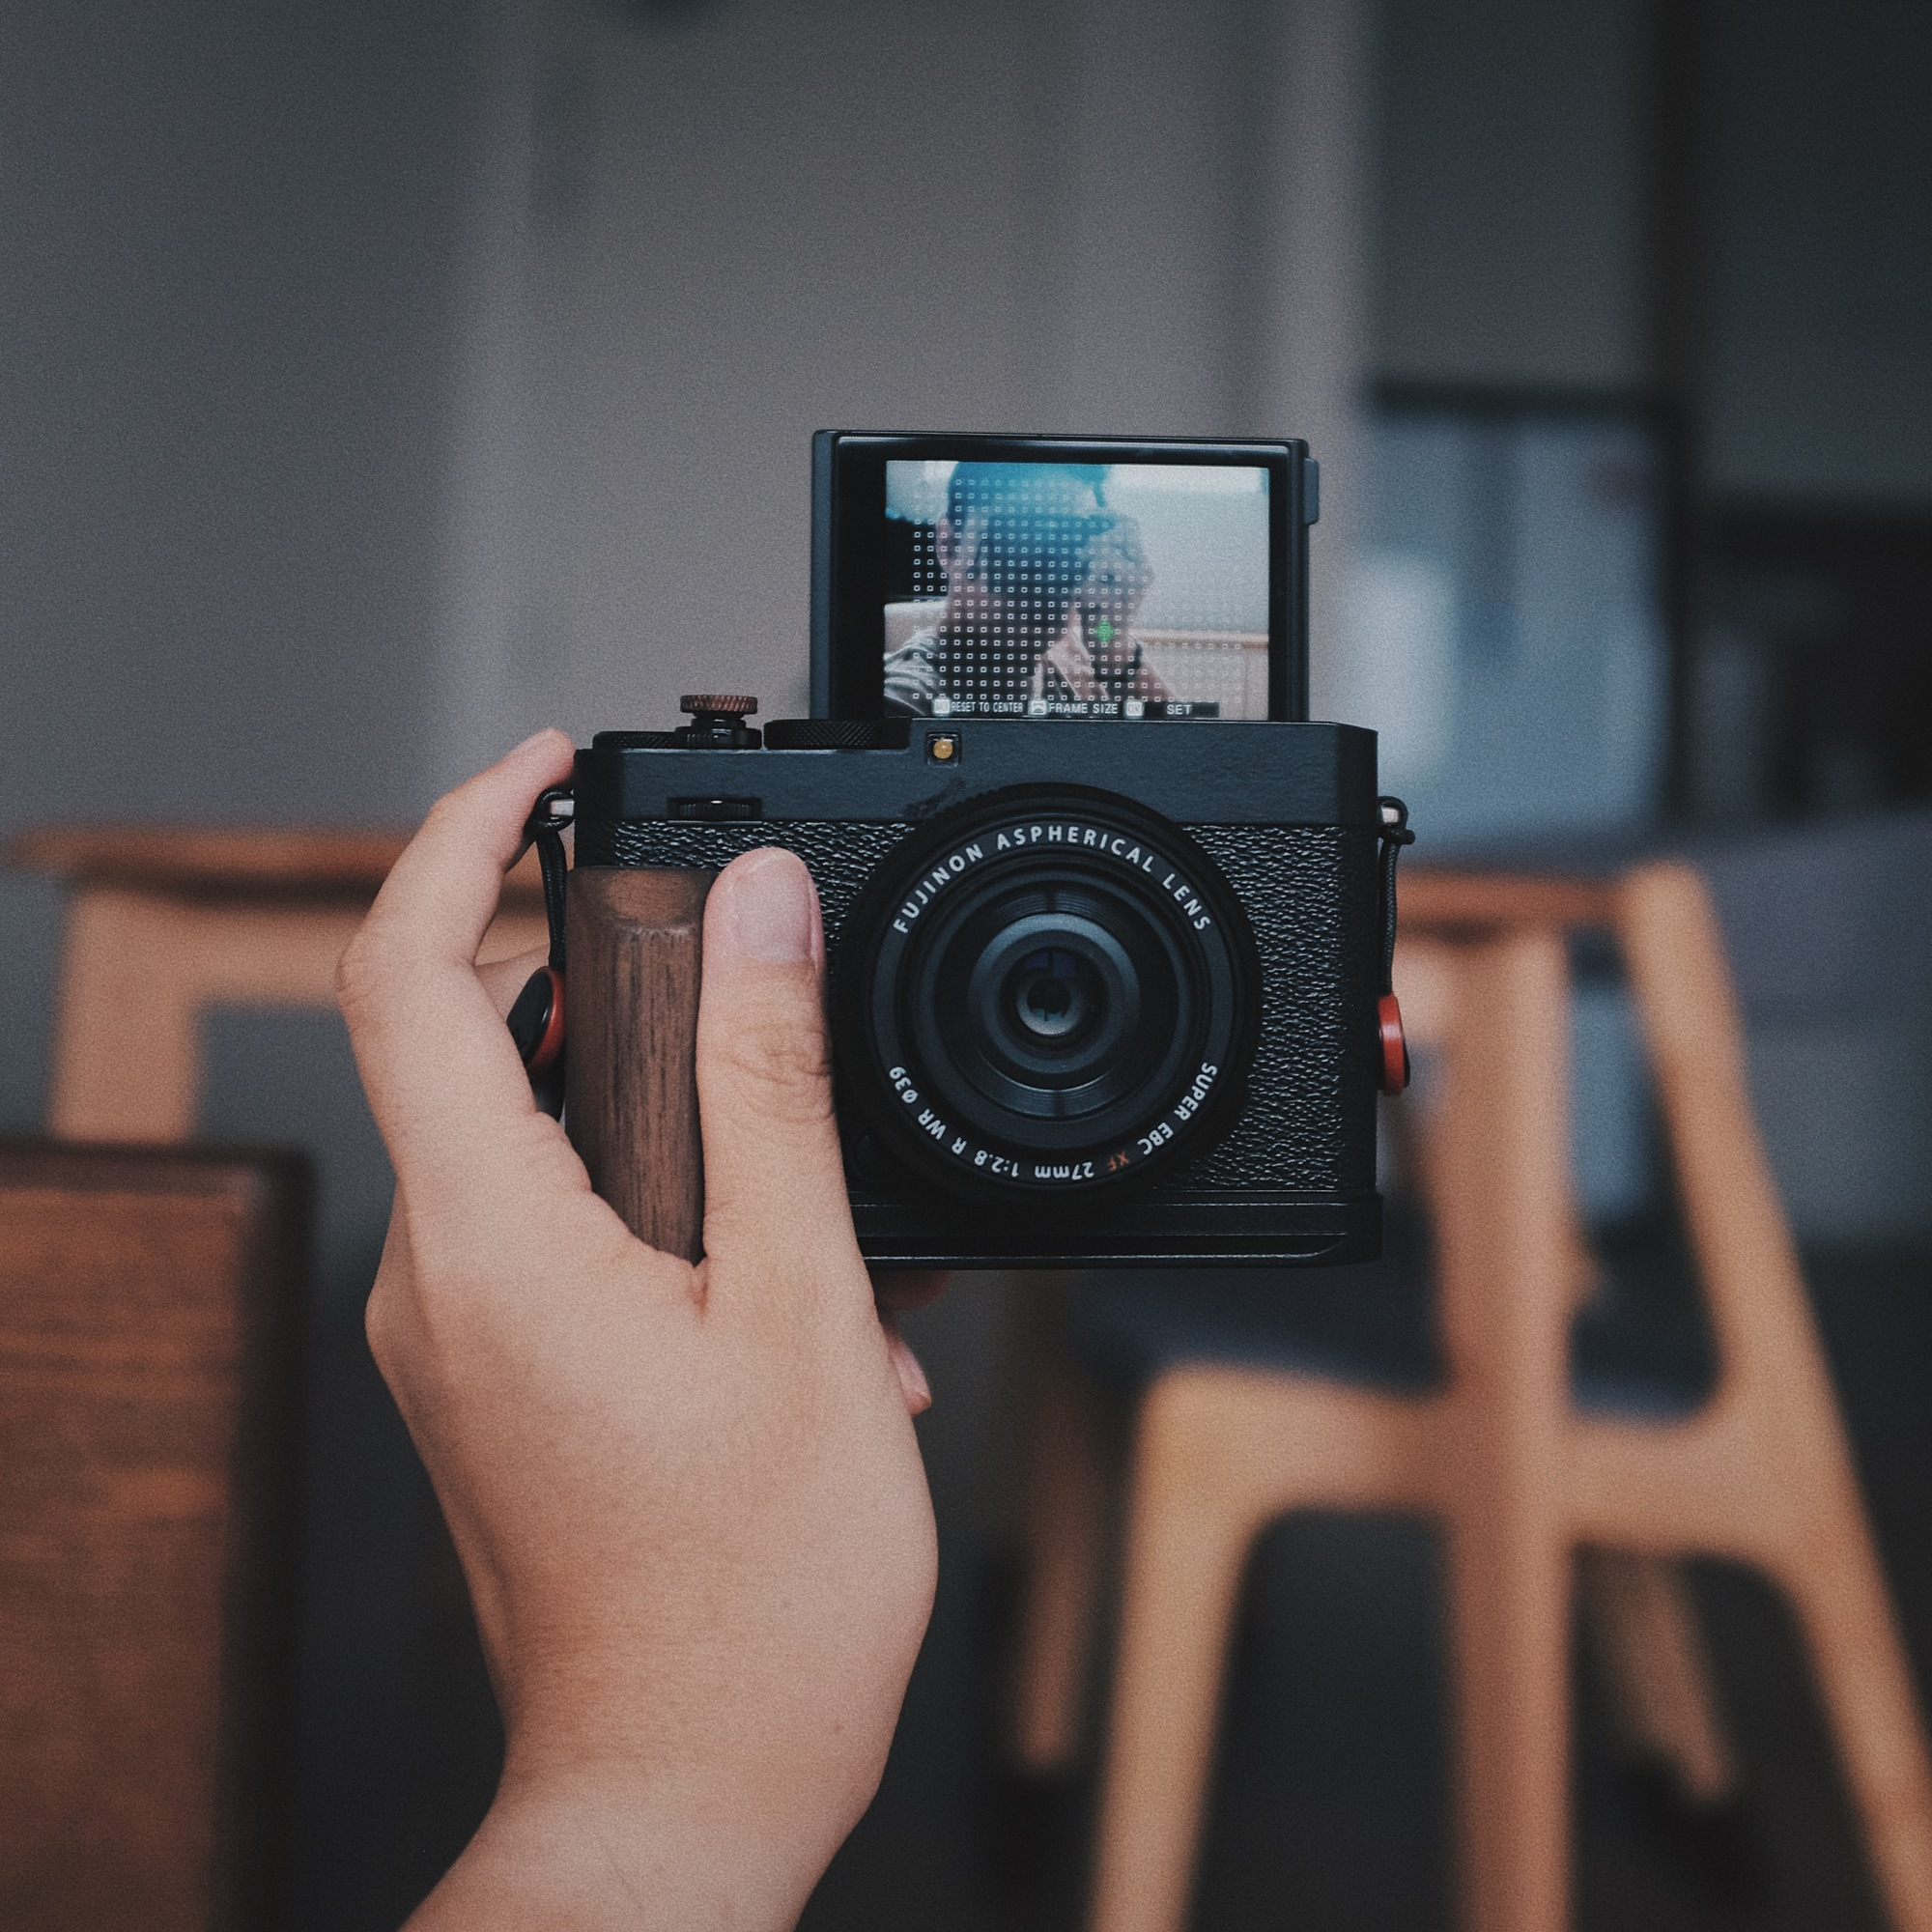
\includegraphics[width=\linewidth]{\envfinaldir/coverpic-prod.jpg}\par
            % \vskip 30pt
            \vfill

            \normalsize\rmfamily\scshape
            \copyright{} The Web Digest Project \hfill\large \envdatestr
        \end{center}
    \end{titlepage}
    % \restoregeometry
}
\newcommand{\simplehref}[1]{%
    \textcolor{blue!80!green}{\href{#1}{#1}}%
}
\renewcommand{\contentsname}{\center\Huge\sffamily\bfseries Contents\par\vskip 20pt}
\newcounter{ipartcounter}
\setcounter{ipartcounter}{0}
\newcommand{\ipart}[1]{
    % \vskip 20pt
    \clearpage
    \stepcounter{ipartcounter}
    \phantomsection
    \addcontentsline{toc}{chapter}{#1}
    % \begin{center}
    %     \Huge
    %     \sffamily\bfseries
    %     #1
    % \end{center}
    % \vskip 20pt plus 7pt
}
\newcounter{ichaptercounter}
\setcounter{ichaptercounter}{0}
\newcommand{\ichapter}[1]{
    % \vskip 20pt
    \clearpage
    \stepcounter{ichaptercounter}
    \phantomsection
    \addcontentsline{toc}{section}{\numberline{\arabic{ichaptercounter}}#1}
    \begin{center}
        \Huge
        \sffamily\bfseries
        #1
    \end{center}
    \vskip 20pt plus 7pt
}
\newcommand{\entrytitlefont}[1]{\subsection*{\raggedright\Large\sffamily\bfseries#1}}
\newcommand{\entryitemGeneric}[2]{
    % argv: title, url
    \parbox{\linewidth}{
        \entrytitlefont{#1}\par\vskip 5pt
        \footnotesize\ttfamily\mdseries
        \simplehref{#2}
    }\vskip 11pt plus 11pt minus 1pt
}
\newcommand{\entryitemGithub}[3]{
    % argv: title, url, desc
    \parbox{\linewidth}{
        \entrytitlefont{#1}\par\vskip 5pt
        \footnotesize\ttfamily\mdseries
        \simplehref{#2}\par\vskip 5pt
        \small\rmfamily\mdseries#3
    }\vskip 11pt plus 11pt minus 1pt
}
\newcommand{\entryitemAp}[3]{
    % argv: title, url, desc
    \parbox{\linewidth}{
        \entrytitlefont{#1}\par\vskip 5pt
        \footnotesize\ttfamily\mdseries
        \simplehref{#2}\par\vskip 5pt
        \small\rmfamily\mdseries#3
    }\vskip 11pt plus 11pt minus 1pt
}
\newcommand{\entryitemHackernews}[3]{
    % argv: title, hnurl, rawurl
    % \parbox{\linewidth}{
    %     \entrytitlefont{#1}\par\vskip 5pt
    %     \footnotesize\ttfamily\mdseries
    %     \simplehref{#3}\par
    %     \textcolor{black!50}{\href{#2}{#2}}
    % }\vskip 11pt plus 11pt minus 1pt
    \begin{minipage}{\linewidth}
            \entrytitlefont{#1}\par\vskip 5pt
            \footnotesize\ttfamily\mdseries
            \simplehref{#3}\par
            \textcolor{black!50}{\href{#2}{#2}}
    \end{minipage}\par\vskip 11pt plus 11pt minus 1pt
}







\begin{document}

\makeheader

\tableofcontents\clearpage




\ipart{Developers}
\ichapter{Hacker News}
\entryitemTwoLinks{Vendors that treat single sign-on as a luxury feature}{https://news.ycombinator.com/item?id=44955457}{https://sso.tax/}

\entryitemTwoLinks{Notion releases offline mode}{https://news.ycombinator.com/item?id=44954665}{https://www.notion.com/help/guides/working-offline-in-notion-everything-you-need-to-know}

\entryitemTwoLinks{D2 (text to diagram tool) now supports ASCII renders}{https://news.ycombinator.com/item?id=44954524}{https://d2lang.com/blog/ascii/}

\entryitemTwoLinks{Emacs as your video-trimming tool}{https://news.ycombinator.com/item?id=44953316}{https://xenodium.com/emacs-as-your-video-trimming-tool}

\entryitemTwoLinks{How we exploited CodeRabbit: From simple PR to RCE and write access on 1M repos}{https://news.ycombinator.com/item?id=44953032}{https://research.kudelskisecurity.com/2025/08/19/how-we-exploited-coderabbit-from-a-simple-pr-to-rce-and-write-access-on-1m-repositories/}

\entryitemTwoLinks{"Remove mentions of XSLT from the html spec"}{https://news.ycombinator.com/item?id=44952185}{https://github.com/whatwg/html/pull/11563}

\entryitemTwoLinks{Positron, a New Data Science IDE}{https://news.ycombinator.com/item?id=44951862}{https://posit.co/blog/positron-product-announcement-aug-2025/}

\entryitemTwoLinks{Why I'm all-in on Zen Browser}{https://news.ycombinator.com/item?id=44951799}{https://werd.io/why-im-all-in-on-zen-browser/}

\entryitemTwoLinks{Without the futex, it's futile}{https://news.ycombinator.com/item?id=44951563}{https://h4x0r.org/futex/}

\entryitemTwoLinks{Critical Cache Poisoning Vulnerability in Dnsmasq}{https://news.ycombinator.com/item?id=44950981}{https://lists.thekelleys.org.uk/pipermail/dnsmasq-discuss/2025q3/018288.html}

\entryitemTwoLinks{'Ad Blocking Is Not Piracy' Decision Overturned by Top German Court}{https://news.ycombinator.com/item?id=44950695}{https://torrentfreak.com/ad-blocking-is-not-piracy-decision-overturned-by-top-german-court-250819/}

\entryitemTwoLinks{UK drops demand for backdoor into Apple encryption}{https://news.ycombinator.com/item?id=44950600}{https://www.theverge.com/news/761240/uk-apple-us-encryption-back-door-demands-dropped}

\entryitemTwoLinks{PyPI Preventing Domain Resurrection Attacks}{https://news.ycombinator.com/item?id=44950091}{https://blog.pypi.org/posts/2025-08-18-preventing-domain-resurrections/}

\entryitemTwoLinks{Custom telescope mount using harmonic drives and ESP32}{https://news.ycombinator.com/item?id=44949895}{https://www.svendewaerhert.com/blog/telescope-mount/}

\entryitemTwoLinks{Google is killing the open web}{https://news.ycombinator.com/item?id=44949857}{https://wok.oblomov.eu/tecnologia/google-killing-open-web/}

\entryitemTwoLinks{BBC witnesses settlers attack on Palestinian farm in West Bank}{https://news.ycombinator.com/item?id=44949264}{https://www.bbc.com/news/articles/cewy88jle0eo}

\entryitemTwoLinks{Prime Number Grid}{https://news.ycombinator.com/item?id=44949162}{https://susam.net/primegrid.html}

\entryitemTwoLinks{How to Build a Medieval Castle}{https://news.ycombinator.com/item?id=44948352}{https://archaeology.org/issues/september-october-2025/features/how-to-build-a-medieval-castle/}

\entryitemTwoLinks{OpenMower – An open source lawn mower}{https://news.ycombinator.com/item?id=44946996}{https://github.com/ClemensElflein/OpenMower}

\entryitemTwoLinks{XZ Utils Backdoor Still Lurking in Docker Images}{https://news.ycombinator.com/item?id=44946783}{https://www.binarly.io/blog/persistent-risk-xz-utils-backdoor-still-lurking-in-docker-images}\ichapter{Phoronix}
\entryitemGeneric{\hskip 0pt{}Tinygrad 0.11 Released With AMD MI350 Support, NVIDIA Blackwell}{https://www.phoronix.com/news/Tinygrad-0.11-Released}

\entryitemGeneric{\hskip 0pt{}Pinned Device Memory Patches For Intel's Multi-GPU "Project Battlematrix" Linux Efforts}{https://www.phoronix.com/news/Intel-Pinned-Device-Memory}

\entryitemGeneric{\hskip 0pt{}Rusticl vs. AMD ROCm Performance On Ryzen AI Max+ "Strix Halo"}{https://www.phoronix.com/review/rocm-rusticl-strix-halo}

\entryitemGeneric{\hskip 0pt{}Linux Adding Detection For BSD's Bhyve Hypervisor To Support 255+ vCPUs}{https://www.phoronix.com/news/Linux-Bhyve-Detection}

\entryitemGeneric{\hskip 0pt{}Apple SoC DT Updates Already Begin Lining Up For Linux 6.18}{https://www.phoronix.com/news/Apple-SoC-DT-Begins-Linux-6.18}

\entryitemGeneric{\hskip 0pt{}Intel Upstreams XeVM Into LLVM}{https://www.phoronix.com/news/Intel-XeVM-MLIR-In-LLVM}

\entryitemGeneric{\hskip 0pt{}Kernel Stack Watch Proposed As New Linux Debugging Tool}{https://www.phoronix.com/news/Kernel-Stack-Watch}

\entryitemGeneric{\hskip 0pt{}New Linux Patches Allow Manipulating Out-Of-Memory Behavior Using BPF}{https://www.phoronix.com/news/Linux-OOM-BPF-Proposal}

\entryitemGeneric{\hskip 0pt{}AMD "GFX1250" To Double The Number Of User SGPRs}{https://www.phoronix.com/news/AMD-GFX1250-32-User-SGPRs}


\ipart{Developers~~~~(zh-Hans)}
\ichapter{Solidot}
\entryitemGeneric{\hskip 0pt{}部分 Docker 镜像仍然包含 XZ Utils 后门 }{https://www.solidot.org/story?sid=82090}

\entryitemGeneric{\hskip 0pt{}软银向英特尔投资 20 亿美元}{https://www.solidot.org/story?sid=82089}

\entryitemGeneric{\hskip 0pt{}MIT 报告称 95\% 的企业生成式 AI 试验失败了}{https://www.solidot.org/story?sid=82088}

\entryitemGeneric{\hskip 0pt{}中国有望在美国之前登陆月球}{https://www.solidot.org/story?sid=82087}

\entryitemGeneric{\hskip 0pt{}英国官员想要阻止儿童使用 VPN 浏览成人内容}{https://www.solidot.org/story?sid=82086}

\entryitemGeneric{\hskip 0pt{}证据显示地球之水起源于彗星}{https://www.solidot.org/story?sid=82085}

\entryitemGeneric{\hskip 0pt{}医生救回几乎``身首离断''患者}{https://www.solidot.org/story?sid=82084}

\entryitemGeneric{\hskip 0pt{}基因改变果蝇的求爱方式}{https://www.solidot.org/story?sid=82083}

\entryitemGeneric{\hskip 0pt{}卫星捕捉到 8.8 级地震所引发海啸的细节}{https://www.solidot.org/story?sid=82082}

\entryitemGeneric{\hskip 0pt{}83\% 的 Python 开发者仍然使用旧版本}{https://www.solidot.org/story?sid=82081}

\entryitemGeneric{\hskip 0pt{}87\% 的游戏开发者在工作中使用 AI}{https://www.solidot.org/story?sid=82080}

\entryitemGeneric{\hskip 0pt{}科学家提议拦截星际彗星 3I/ATLAS}{https://www.solidot.org/story?sid=82079}

\entryitemGeneric{\hskip 0pt{}大众想要司机支付月费以解锁更高的动力}{https://www.solidot.org/story?sid=82078}

\entryitemGeneric{\hskip 0pt{}水星因热量流失不端缩小}{https://www.solidot.org/story?sid=82077}

\entryitemGeneric{\hskip 0pt{}黑猩猩从母亲而不是父亲学会交流模式}{https://www.solidot.org/story?sid=82076}

\entryitemGeneric{\hskip 0pt{}英国监管机构调查 4chan 考虑罚款 2 万英镑}{https://www.solidot.org/story?sid=82075}

\entryitemGeneric{\hskip 0pt{}Microsoft Store 应用将强制性自动更新}{https://www.solidot.org/story?sid=82074}

\entryitemGeneric{\hskip 0pt{}Meta 的 AI 规则允许聊天机器人与儿童调情}{https://www.solidot.org/story?sid=82073}

\entryitemGeneric{\hskip 0pt{}AO3 中文同人作品突破百万篇}{https://www.solidot.org/story?sid=82072}

\entryitemGeneric{\hskip 0pt{}微软最新更新可能会导致硬盘故障}{https://www.solidot.org/story?sid=82071}\ichapter{V2EX}
\entryitemGeneric{\hskip 0pt{}[Google] 小米手机怎么打开 google 设置}{https://www.v2ex.com/t/1153577}

\entryitemGeneric{\hskip 0pt{}[生活] 女朋友发火了}{https://www.v2ex.com/t/1153576}

\entryitemGeneric{\hskip 0pt{}[游戏] 非常佩服游戏科学的决定}{https://www.v2ex.com/t/1153575}

\entryitemGeneric{\hskip 0pt{}[游戏] 游戏科学新作《黑神话·钟馗》}{https://www.v2ex.com/t/1153574}

\entryitemGeneric{\hskip 0pt{}[问与答] 春秋上个月刚出的 gopay 有了解的吗?看起来类似于野卡}{https://www.v2ex.com/t/1153573}

\entryitemGeneric{\hskip 0pt{}[OpenWrt] 有没有 在 Openwrt 中使用 strongswan 成功配置 IPSec/IKEv2 客户模式的吗?指点下}{https://www.v2ex.com/t/1153572}

\entryitemGeneric{\hskip 0pt{}[随想] 完了,玩游戏玩到现在,感觉要被开除了😭}{https://www.v2ex.com/t/1153571}

\entryitemGeneric{\hskip 0pt{}[程序员] 深夜 GFW 疑似大规模干扰 443 端口连接}{https://www.v2ex.com/t/1153568}

\entryitemGeneric{\hskip 0pt{}[分享发现] 世纪大断网吗?}{https://www.v2ex.com/t/1153567}

\entryitemGeneric{\hskip 0pt{}[问与答] 好奇为什么代理访问海外 443 也会阻断?}{https://www.v2ex.com/t/1153566}

\entryitemGeneric{\hskip 0pt{}[宽带症候群] 临时工别三天两头杀自己人的网络了好不好}{https://www.v2ex.com/t/1153565}

\entryitemGeneric{\hskip 0pt{}[生活] 1781 - 分享初恋并且是网恋+暗恋的故事}{https://www.v2ex.com/t/1153564}

\entryitemGeneric{\hskip 0pt{}[VPS] 中国大陆与海外的 443 端口全部挂了}{https://www.v2ex.com/t/1153563}

\entryitemGeneric{\hskip 0pt{}[宽带症候群] 现在从国外访问国内的网站,全部无法访问, https 阻断}{https://www.v2ex.com/t/1153562}

\entryitemGeneric{\hskip 0pt{}[VPS] 深夜突发所有的海外 443 端口被阻断,你的 vps 还好吗}{https://www.v2ex.com/t/1153561}

\entryitemGeneric{\hskip 0pt{}[全球工单系统] 刚刚 aliyun 上的国内网站全打不开了,国内打开正常,坐标新加坡}{https://www.v2ex.com/t/1153560}

\entryitemGeneric{\hskip 0pt{}[VXNA] 申请站长收录我的博客}{https://www.v2ex.com/t/1153558}

\entryitemGeneric{\hskip 0pt{}[程序员] 框架选型问题 React Native、Flutter、uniappx?}{https://www.v2ex.com/t/1153555}

\entryitemGeneric{\hskip 0pt{}[信息安全] 发现谷歌地图有 xss,请问该去哪提交给厂商?}{https://www.v2ex.com/t/1153554}

\entryitemGeneric{\hskip 0pt{}[分享创造] 一个多平台英语单词收集工具,从阅读中积累词汇,打造个人高频词库,支持同步到欧路/墨墨/扇贝生词本}{https://www.v2ex.com/t/1153553}

\entryitemGeneric{\hskip 0pt{}[程序员] 拒绝 AI Coding 焦虑}{https://www.v2ex.com/t/1153551}

\entryitemGeneric{\hskip 0pt{}[分享创造] 商品低价提醒的软件}{https://www.v2ex.com/t/1153550}

\entryitemGeneric{\hskip 0pt{}[全球工单系统] 淘宝个性化推荐关闭的选项是摆设?}{https://www.v2ex.com/t/1153549}

\entryitemGeneric{\hskip 0pt{}[深圳] 深圳租房求助}{https://www.v2ex.com/t/1153546}

\entryitemGeneric{\hskip 0pt{}[Solana] 需要少量 sol}{https://www.v2ex.com/t/1153545}

\entryitemGeneric{\hskip 0pt{}[程序员] 视频生成的模型怎么编写 prompt 最好?}{https://www.v2ex.com/t/1153543}

\entryitemGeneric{\hskip 0pt{}[酷工作] [北、上、深] 百亿量化私募 C++/ Python /Go/数据开发/测试/运维/算法}{https://www.v2ex.com/t/1153542}

\entryitemGeneric{\hskip 0pt{}[天黑以后] 20250819 午夜俱乐部}{https://www.v2ex.com/t/1153541}

\entryitemGeneric{\hskip 0pt{}[分享创造] 分享一个 Claude Code 的配置助手工具站}{https://www.v2ex.com/t/1153540}

\entryitemGeneric{\hskip 0pt{}[Java] cursor 替换 idea 作为 Java 主力开发工具}{https://www.v2ex.com/t/1153539}

\entryitemGeneric{\hskip 0pt{}[程序员] 在大模型以及 AI IDE 的辅助下,疑似看``源码''从一个看似比较高级的事情沦为了``体力活儿''}{https://www.v2ex.com/t/1153536}

\entryitemGeneric{\hskip 0pt{}[前端开发] 我开源了一个可能是功能最全的表单库-支持 Angular,Vue,React,Svelte,Solid}{https://www.v2ex.com/t/1153535}

\entryitemGeneric{\hskip 0pt{}[Pixel] 折磨人的"VPN by Google"}{https://www.v2ex.com/t/1153534}

\entryitemGeneric{\hskip 0pt{}[远程工作] unity 全栈(远程)}{https://www.v2ex.com/t/1153533}

\entryitemGeneric{\hskip 0pt{}[程序员] 苦于 CLI 没有 LLM 可用,所以自己写轮子}{https://www.v2ex.com/t/1153532}

\entryitemGeneric{\hskip 0pt{}[Mac 游戏] 求一个 mac 版本的实况足球 8}{https://www.v2ex.com/t/1153531}

\entryitemGeneric{\hskip 0pt{}[问与答] windows 系统更新导致 ssd 变砖的情况有人遇到了么?}{https://www.v2ex.com/t/1153530}

\entryitemGeneric{\hskip 0pt{}[分享发现] Apple 时钟的滚轮不是循环的}{https://www.v2ex.com/t/1153529}

\entryitemGeneric{\hskip 0pt{}[问与答] 各位都是如何使用亚马逊 ec2 服务器的}{https://www.v2ex.com/t/1153528}

\entryitemGeneric{\hskip 0pt{}[Python] 仿照 uv 写了个包管理器,用过的都说好}{https://www.v2ex.com/t/1153527}

\entryitemGeneric{\hskip 0pt{}[分享创造] 用 GPT-5 + Codex 打磨了一下两年前的一个点子💡}{https://www.v2ex.com/t/1153526}

\entryitemGeneric{\hskip 0pt{}[分享创造] 3 年前,我在考研,我就希望有这样的软件,可以把需要记忆的材料转为记忆卡片。现在我毕业了,我做了一个软件,尝试用 AI 去做这件事。}{https://www.v2ex.com/t/1153525}

\entryitemGeneric{\hskip 0pt{}[分享创造] 借 wplace 灵感,用 AI 做了个 WebMap}{https://www.v2ex.com/t/1153524}

\entryitemGeneric{\hskip 0pt{}[Apple] iPad 和 iPhone 上如何在 obsidian 上安装第三方字体?}{https://www.v2ex.com/t/1153523}

\entryitemGeneric{\hskip 0pt{}[程序员] 你们会在项目中使用 Emoji 么?比如打印日志什么的}{https://www.v2ex.com/t/1153522}

\entryitemGeneric{\hskip 0pt{}[酷工作] [杭州] 坐标阿里云,招聘 k8s 研发工程师}{https://www.v2ex.com/t/1153521}

\entryitemGeneric{\hskip 0pt{}[分享发现] 新主板烧了两块硬盘}{https://www.v2ex.com/t/1153520}

\entryitemGeneric{\hskip 0pt{}[问与答] 各位给孩子练英语听力,用什么设备?}{https://www.v2ex.com/t/1153519}

\entryitemGeneric{\hskip 0pt{}[程序员] cursor 好用还是 trae 好用?}{https://www.v2ex.com/t/1153517}

\entryitemGeneric{\hskip 0pt{}[程序员] 现阶段 AI 编程真的可行么?}{https://www.v2ex.com/t/1153516}


\ipart{Generic News}







\clearpage
\leavevmode\vfill
\footnotesize

Copyright \copyright{} 2023-2025 Neruthes and other contributors.

This document is published with CC BY-NC-ND 4.0 license.

The entries listed in this newsletter may be copyrighted by their respective creators.

This newsletter is generated by the Web Digest project.

The newsletters are also delivered via Telegram channel \CJKunderline{\href{https://t.me/webdigestchannel}{https://t.me/webdigestchannel}}.\\
RSS feed is available at \CJKunderline{\href{https://webdigest.pages.dev/rss.xml}{https://webdigest.pages.dev/rss.xml}}.

This newsletter is available in PDF at
\CJKunderline{\href{https://webdigest.pages.dev/}{https://webdigest.pages.dev/}}.

The source code being used to generate this newsletter is available at\\
\CJKunderline{\href{https://github.com/neruthes/webdigest}{https://github.com/neruthes/webdigest}}.

This newsletter is also available in
\CJKunderline{\href{http://webdigest.pages.dev/readhtml/\envyear/WebDigest-20250820.html}{HTML}} and
\CJKunderline{\href{https://github.com/neruthes/webdigest/blob/master/markdown/\envyear/WebDigest-20250820.md}{Markdown}}.


\coverpic{https://unsplash.com/photos/woman-wearing-striped-button-up-shirt-bhE9jEgqZ04}{roland deason}


\end{document}
